\subsection{Component-Bus-System-Property (JEM)}\label{cbsp}

Component-Bus-System-Property, kurz CBSP, ist ein leichtgewichtiger Ansatz um Anforderungen und Architektur mit Hilfe von Zwischenmodellen in Übereinstimmung zu bringen \cite{Gru01}. Dazu wird iterativ aus den Anforderungen ein CBSP Modell gebildet, welches Anforderungs- und Architektur-Modellelemente miteinander verknüpft. \\

\subsubsection{Ziele der Methode}

Der CBSP Ansatz hilft Software-Architekten dabei Architekturelemente wie Komponenten und Konnektoren, Architektur Eigenschaften, Abhängigkeiten zwischen diesen Elementen und passende Architekturstile zu finden. Dabei unterstützt das CBSP den Software-Architekten dabei folgende Herausforderungen, um Anforderungen und Architektur in Übereinstimmung zu bringen, zu behandeln: \\

\begin{itemize}
\item \textit{Überbrückung unterschiedlicher Formalitätsebenen}: Das Zwischenmodell von CBSP reduziert die Semantische Lücke zwischen meist informell in natürlicher Sprache gehaltenen Anforderungen auf einer höheren Abstraktionsebene und eher formell gehaltenen Architekturbeschreibungen \cite{Gru01}.
\item \textit{Modellierung nicht-funktionaler Anforderungen}: CBSP ermöglicht, die sonst schwere Modellierung von nicht-funktionalen Anforderungen als Architekturmodell sowohl auf der System- wie auch der Architekturebene \cite{Gru01}. 
\item \textit{Aufrechterhaltung evolutionärer Konsistenz}: Aufrechterhaltung von Konsistenz und Nachverfolgbarkeit ist ein schwieriges Unterfangen, da eine einzelne Anforderung mehrere architektonische Anliegen betreffen kann und ein einzelnes Architekturelement typischerweise mehrere Beziehungen zu verschiedenen Anforderungen hat \cite{Gru01}. Diese Schwierigkeiten werden vom CBSP Zwischenmodell behoben.
\item \textit{Unvollständige Modelle und iterative Entwicklung}: Das CBSP Zwischenmodell benötigt auf Grund seines iterativen Vorgehensmodells keine von Beginn an vollständige Anforderungsspezifikation. Desweiteren können bestimmte Anforderungen erst vollständig verstanden werden, wenn die Software-Architektur modelliert oder sogar partiell implementiert wurde \cite{Gru01}.
\item \textit{Größe und Komplexität Behandeln}: Großsysteme müssen meist hunderte bis tausende von Anforderungen erfüllen. Da CBSP sich in jeder Iteration nur mit einem Teil der architektonisch relevanten Anforderungen beschäftigt kann es diese Komplexität beherschen und den Fokus erhöhen. Jede Aktivität von CBSP befasst sich mit der Filterung von Anforderungen oder dem Zusammenfassen mehrerer Anforderungen in eine \cite{Gru01}.
\item \textit{Verschiedene Stakeholder mit unterschiedlichen Interessen}: Anforderungen und Architektur in Einklang zu bringen ist auch ein Prozess in welchem heterogene Stakeholder mit widersprüchlichen Zielen, Erwartungen und Terminologien involviert sind. CBSP versucht hier die richtige Balance zwischen diesen abweichenden Interessen zu finden indem es wichtige Stakeholder involviert \cite{Gru01}. \\
\end{itemize}

Um bei der Bewältigung dieser Herausforderungen zu unterstützen bietet das CBSP: \\

\begin{itemize}
\item einen leichtgewichtigen Ansatz Anforderungen zu verfeinern durch die Bereitstellung eines kleinen erweiterbaren Sets von Architektur Schlüsselkomponenten, 
\item einen Mechanismus um die Anzahl relevanter Anforderungen zu reduzieren und auf die relevantesten ASFRs zu fokussieren, 
\item Beteiligung von wichtigen Stakeholdern, 
\item einen regulierbaren Voting-Mechanismus um Konflikte und unterschiedliche Auffassungen zwischen Architekten zu beheben und
\item Toolunterstützung für bestimmte Schritte des Ansatzes \cite{Gru01}. \\
\end{itemize}

\subsubsection{Funktionsweise der Methode}

Das CBSP erweitert, wie in Figur \ref{fig_cbsp_model} zu sehen ist, den Gedanken des Twin-Peaks Modells. Das Zwischenmodell des CBSP verknüpft die Anforderungen mit der Architektur. Das iterative Vorgehen kann dabei sogar auf verschiedenen Detail- bzw. Abstraktionsstufen angewandt werden \cite{Gru01}. 
Um das Vorgehen genauer verstehen zu können wird zunächst die Taxonomie des CBSP betrachtet. \\

\begin{figure}[h]
	\centering
	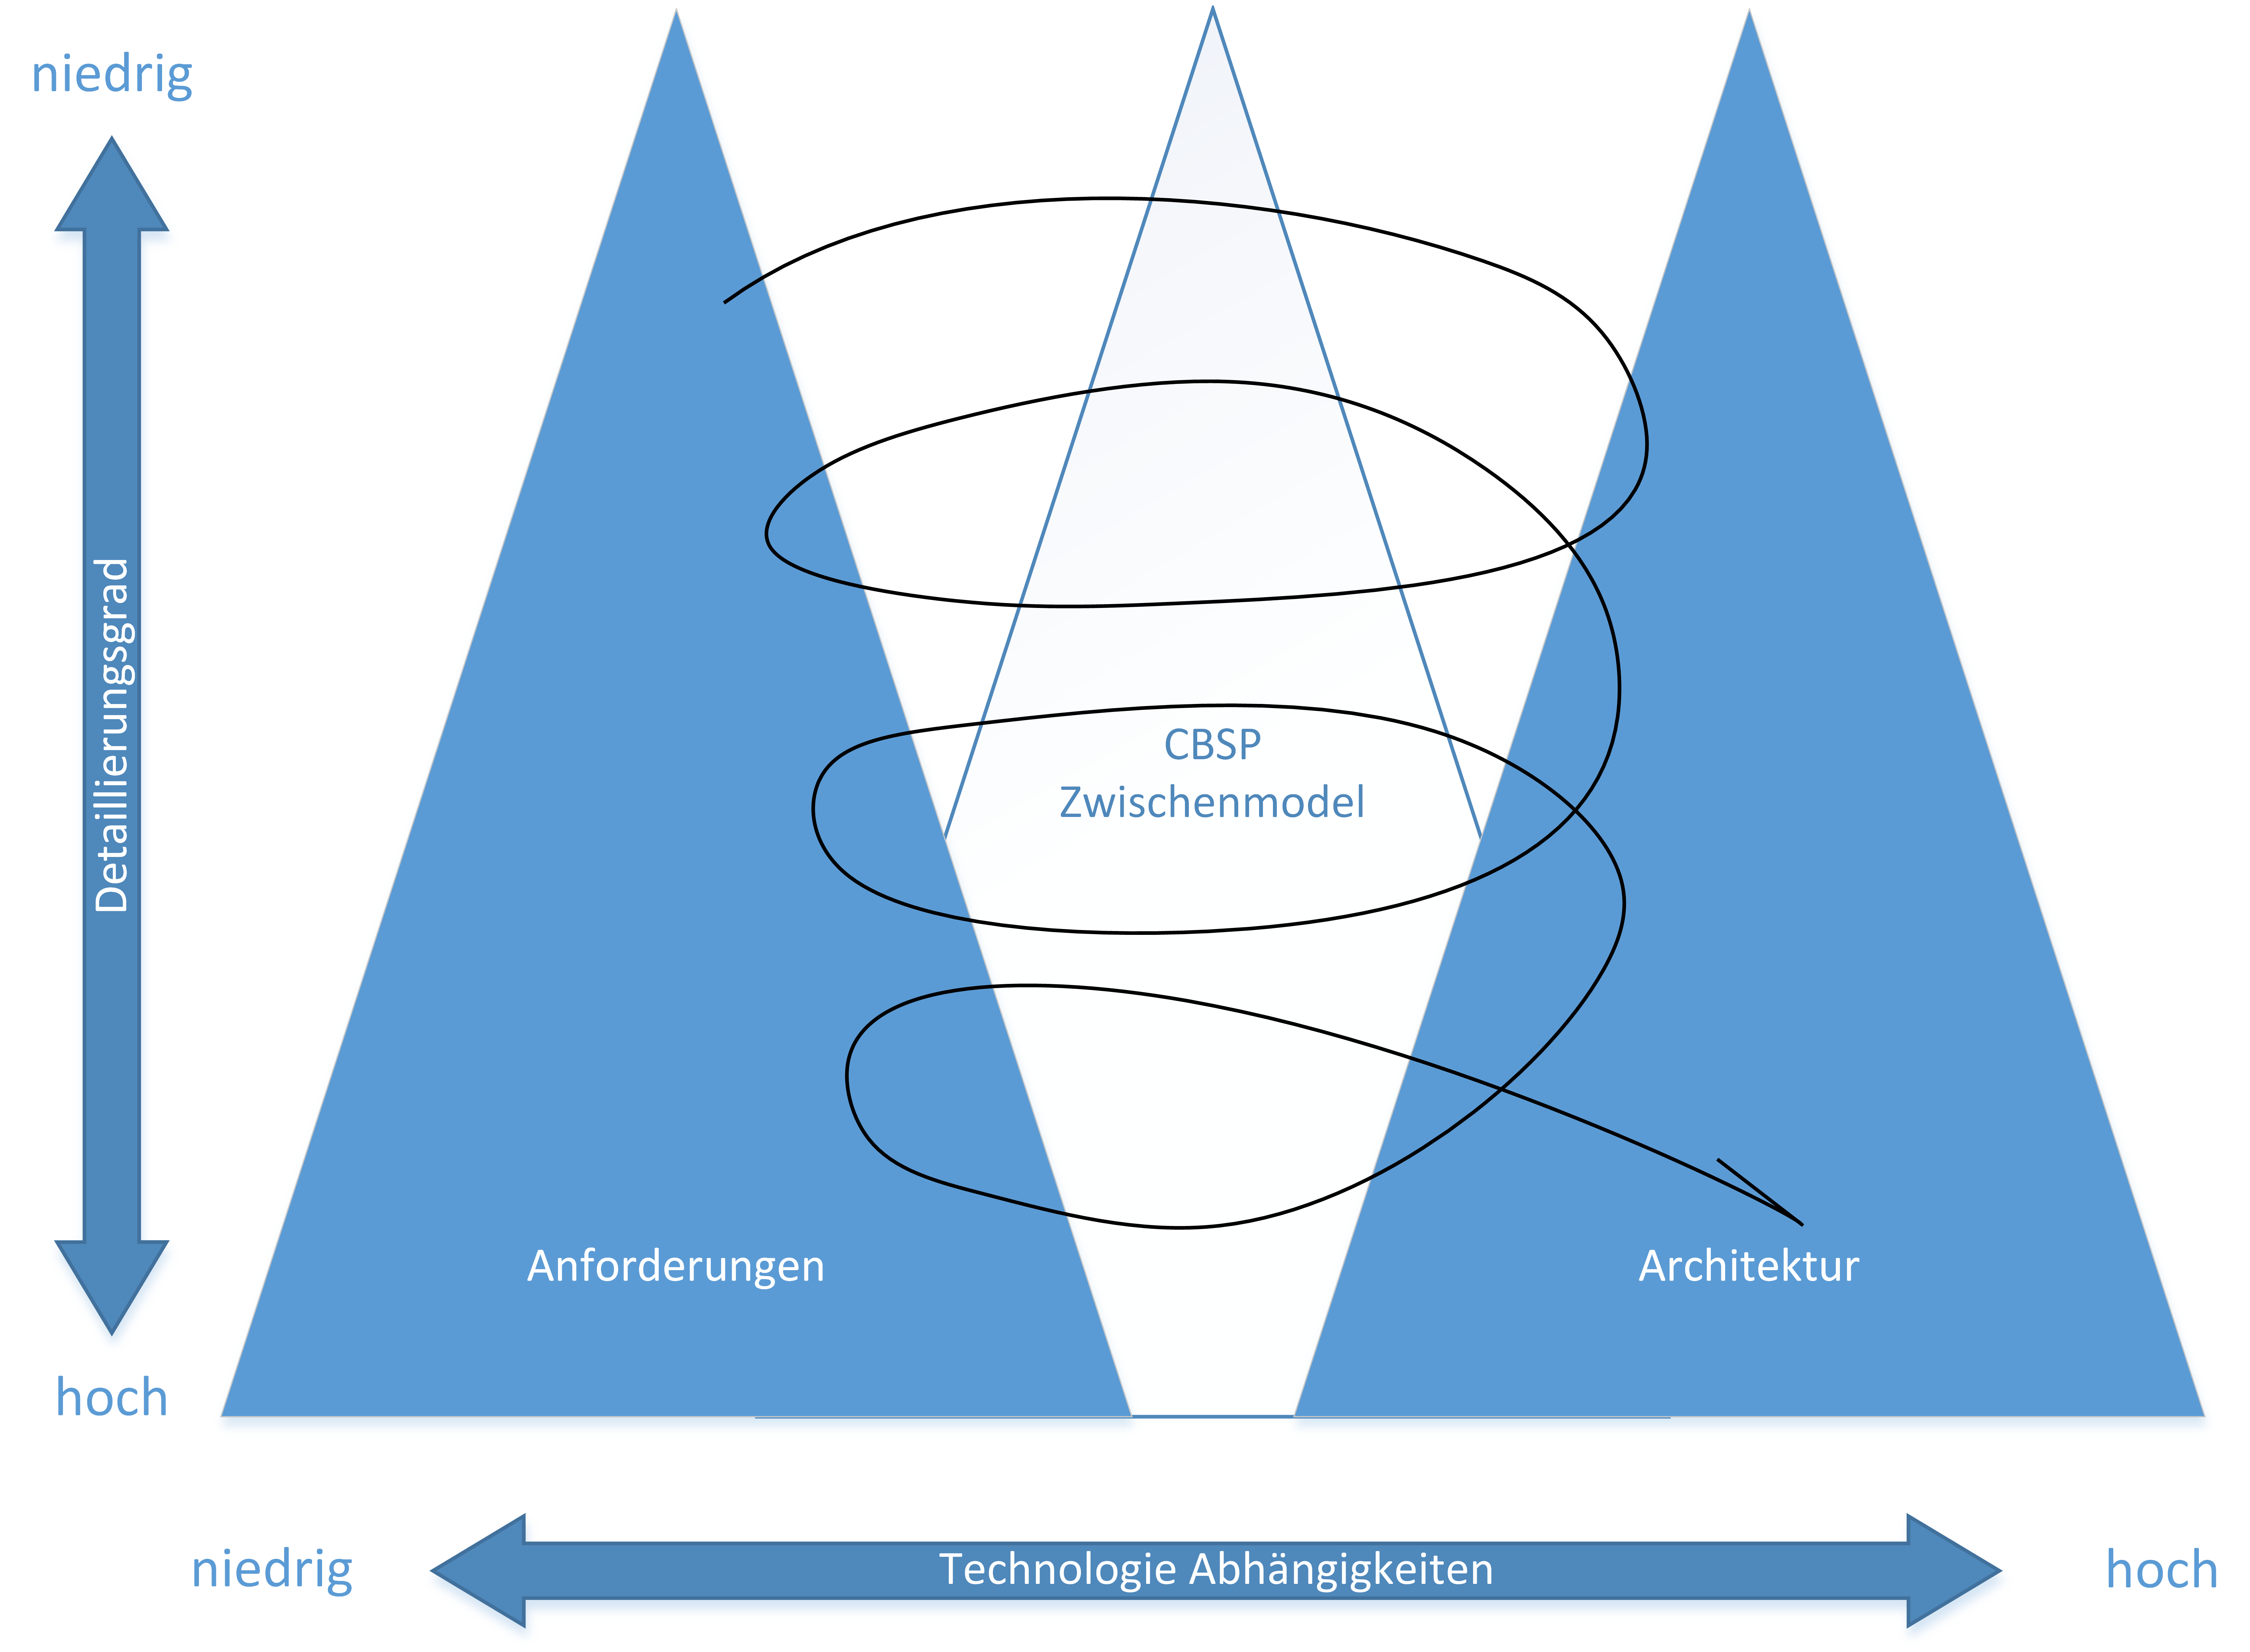
\includegraphics[scale=0.5]{cbsp_model2.png} 
	\caption{CBSP Modell Kontext \cite{Gru01}}
	\label{fig_cbsp_model}
\end{figure}

\textbf{CBSP Taxonomie:}
Das Metamodell von CBSP beinhaltet die Basiskonstrukte einer Architektur und ist in sechs Dimensionen aufgeteilt: \\

\begin{itemize}
\item[1.] \textit{C}: sind Elemente, welche individuelle Komponenten der Software-Architektur beschreiben oder involvieren. Diese sind in Datenkomponenten (C\textsubscript{D}) und Verarbeitungskomponenten (C\textsubscript{P}) unterteilt. So könnte beispielsweise die Anforderung: \\
	\textit{R: Benutzern das direkte manipulieren von Kalkulationstabellen erlauben.} \\
	in folgende CBSP Modellelemente verfeinert werden: \\
	\textit{C\textsubscript{P}: UI Komponente für Kalkulationstabellen Manipulation.} \\
	\textit{C\textsubscript{D}: Daten für Kalkulationstabellen.}  \cite{Gru01}
\item[2.] \textit{B}: sind Elemente, welche Konnektoren beschreiben. Zum Beispiel: \\
	\textit{R: Manipulierte Daten in Kalkulationstabellen muss im Dateisystem gespeichert werden.} \\
	kann in folgendes CBSP Modellelement verfeinert werden: \\
	\textit{B: Konnektor der die Interaktion zwischen UI und Persistenz-Komponenten ermöglicht.} \cite{Gru01}
\item[3.] \textit{S}: sind Elemente, welche systemweite Features beschreiben oder solche, die zu einer größeren Untermenge von Komponenten und Konnektoren passen. Zum Beispiel: \\
	\textit{R: Der Benutzer soll angemessene Filter und Visualisierungen auswählen können.} \\
	kann in folgendes CBSP Modellelement verfeinert werden: \\
	\textit{S: Das System soll eine strikte Trennung von Datenhaltungs-, -Bearbeitungs- und -Visualisierungs-Komponenten vornehmen.} \cite{Gru01}
\item[4.] \textit{CP}: sind Elemente, welche Eigenschaften, wie Zuverlässigkeit, Portabilität, Skalierbarkeit, Anpassbarkeit und Erweiterbarkeit, von Daten- oder Verarbeitungskomponenten beschreiben. Zum Beispiel: \\
	\textit{R: Das Benutzer soll die Daten entfernt mit minimale wahrgenommener Latenz visualisieren können.} \\
	kann in folgendes CBSP Modellelement verfeinert werden: \\
	\textit{CP: Die Datenvisualisierungs-Komponente soll effizient sein und inkrementelle Updates unterstützen.} \cite{Gru01}
\item[5.] \textit{BP}: sind Elemente, welche Eigenschaften von Konnektoren beschreiben. Zum Beispiel: \\
	\textit{R: Updates für Systemfunktionen sollen mit minimaler Ausfallzeit möglich sein.} \\
	kann in folgendes CBSP Modellelement verfeinert werden: \\
	\textit{BP: Robuste Konnektoren sollen zur Verfügung gestellt werden, um das Hinzufügen und Entfernen von Laufzeitkomponenten zu erleichtern.} \cite{Gru01}
\item[6.] \textit{SP}: sind Elemente, welche systemweite Eigenschaften bzw. Eigenschaften von Subsystemen beschreiben. Zum Beispiel: \\
	\textit{R: Die Daten der Kalkulationstabellen müssen verschlüsselt werden bevor sie über das Netzwerk versandt werden.} \\
	kann in folgendes CBSP Modellelement verfeinert werden: \\
	\textit{SP: Das System soll sicher sein.} \cite{Gru01} \\
\end{itemize}

Aus diesen Elementen wird das CBSP Zwischenmodell aufgebaut. Das Metamodell zu diesen Elementen ist in Figur \ref{fig_cbsp_meta_model} dargestellt. Jedes CBSP Artefakt beschreibt eine architekturrelevantes Anliegen und beschreibt eine frühe Architekturentscheidung des zu erstellenden Systems \cite{Gru01}. \\

Von einer Anforderung zu einem CBSP Element kann eine Verfeinerung, siehe Beispiel (5), oder Generalisierung, siehe Beispiel (6), erfolgen. Diese beiden möglichen Anpassungen basieren auf Notwendigkeiten, welche durch bestimmte Eigenschaften des zu erstellenden Systems, Charakteristika der Anwendungsdomäne oder Hintergrund und Erfahrung des Software-Architekten, erwachsen \cite{Gru01}. Da es für Verfeinerung und Generalisierung keine allgemeinen formalen Regeln gibt, ist es häufig notwendig hierfür den Kunden bzw. die Stakeholder zu konsultieren \cite{Gru01}. 

\begin{figure}[h]
	\centering
	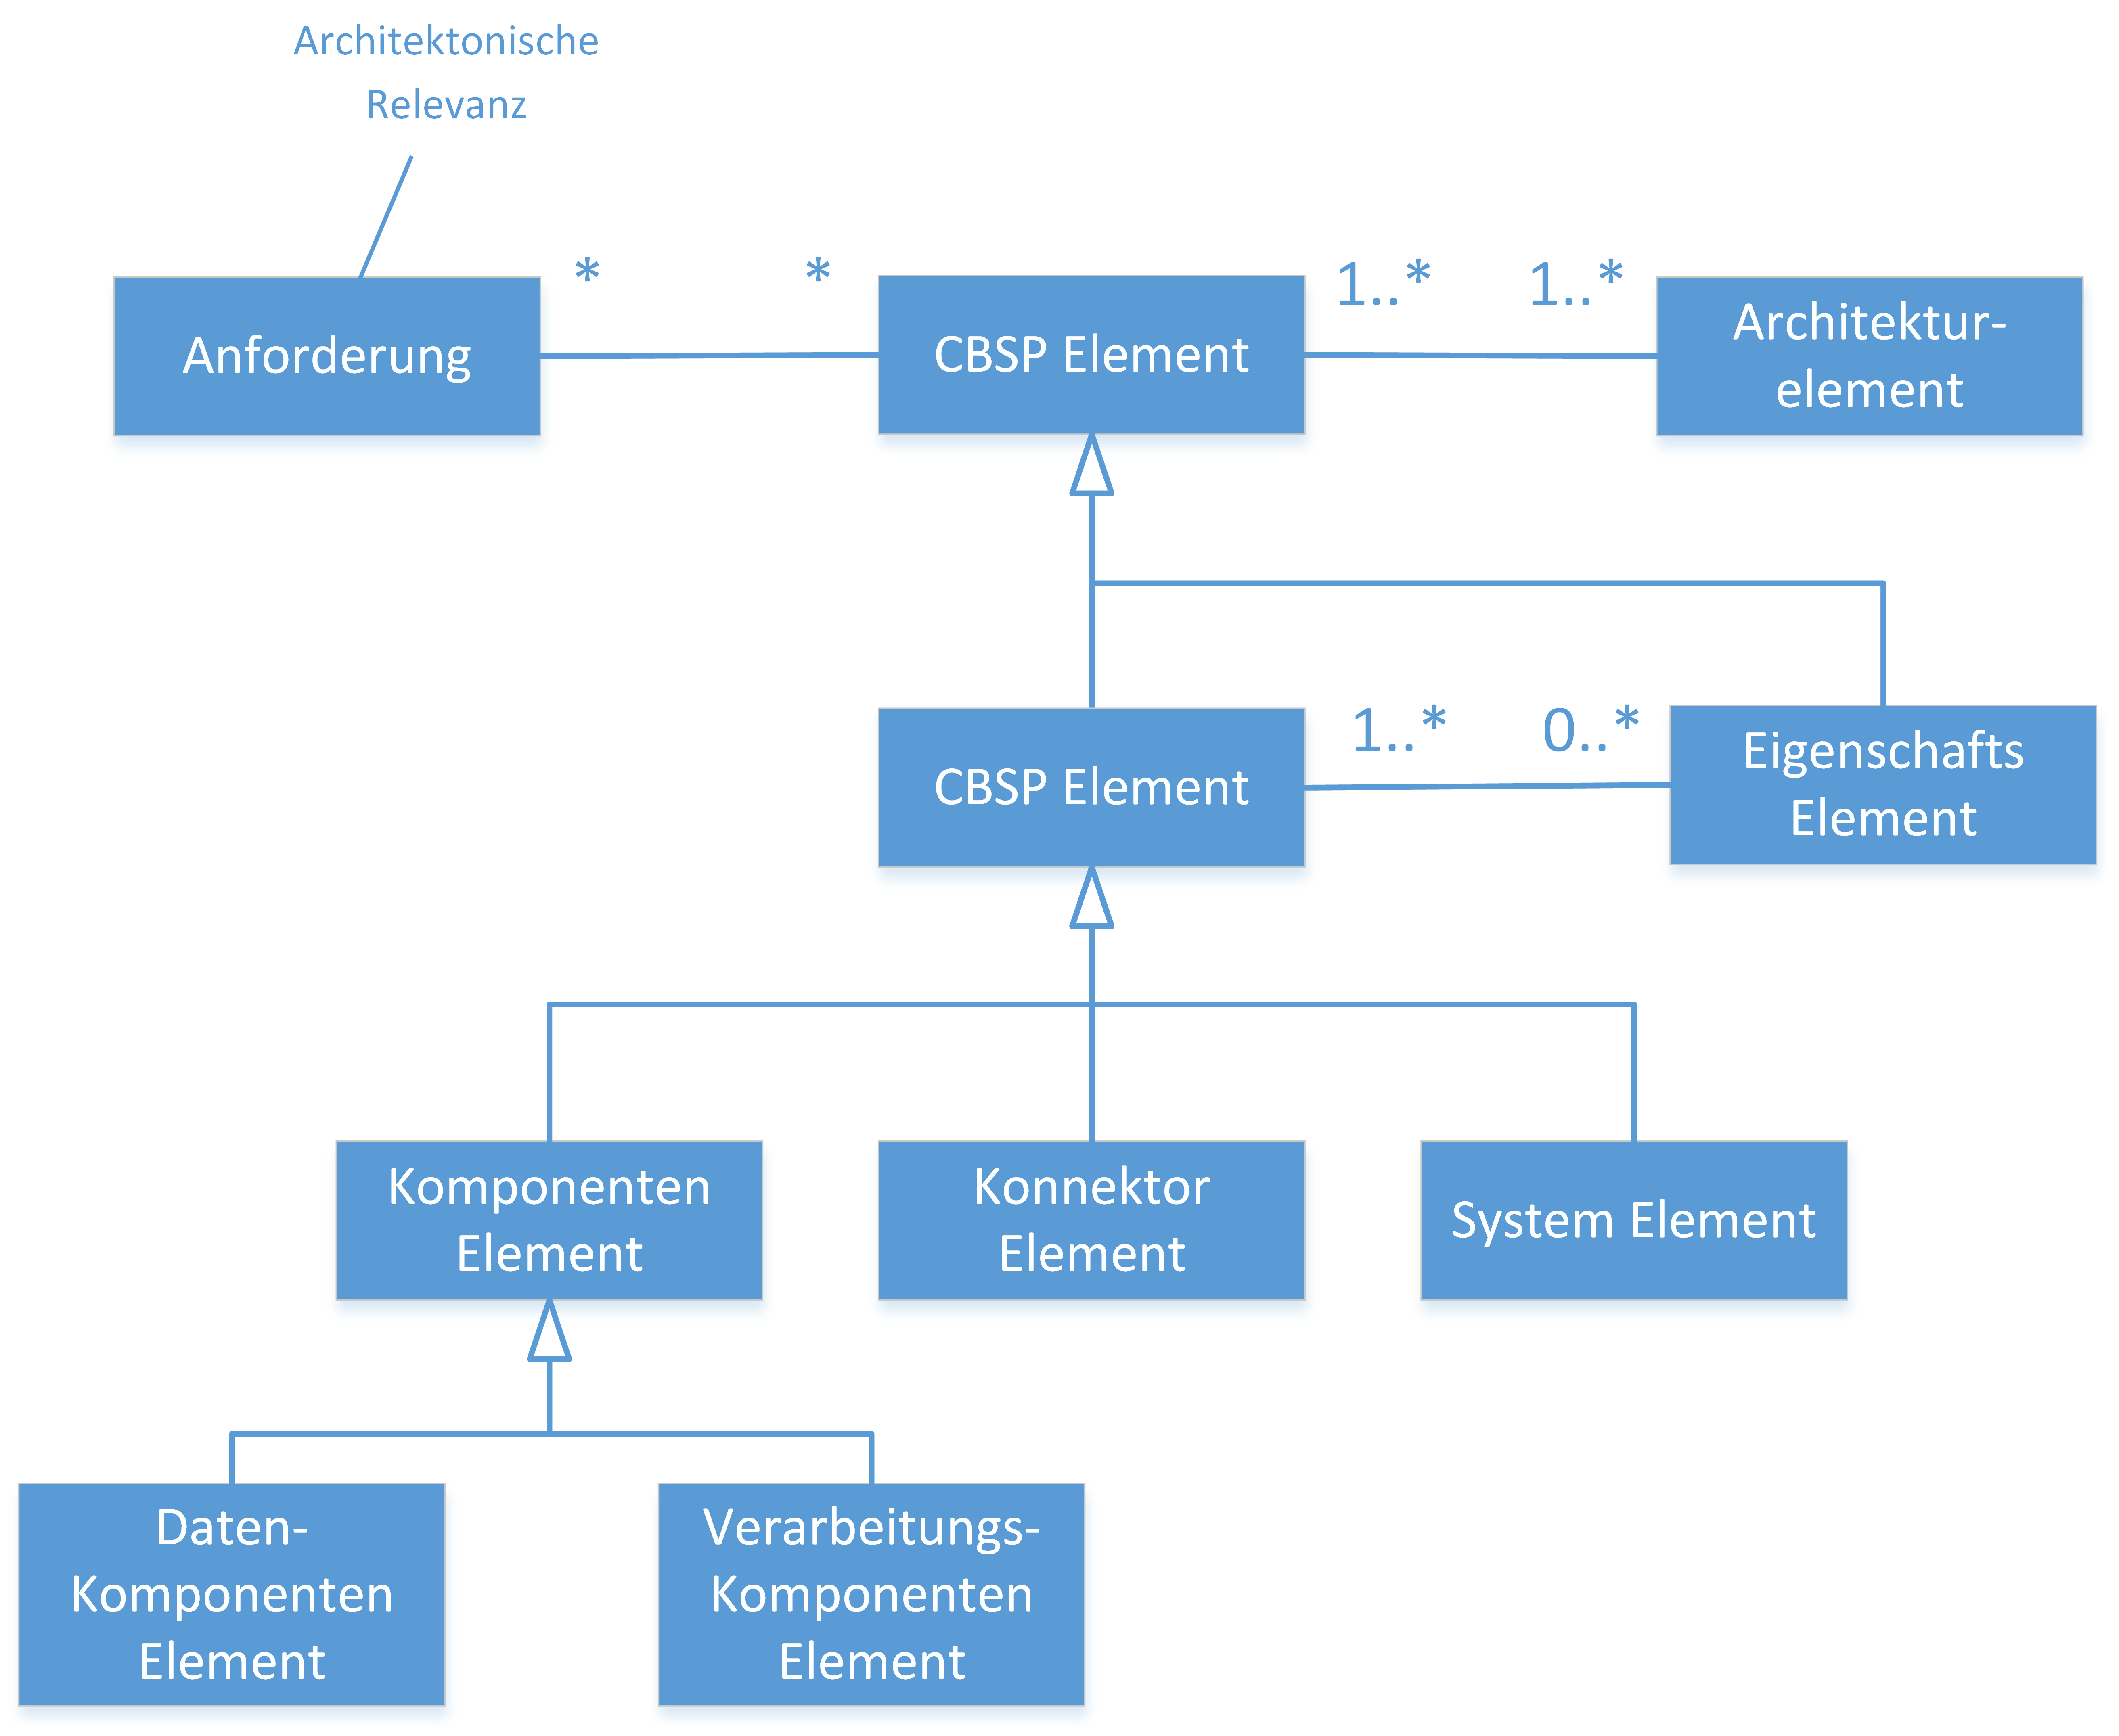
\includegraphics[scale=0.6]{cbsp_meta_model.png} 
	\caption{CBSP Metamodell \cite{Gru01}}
	\label{fig_cbsp_meta_model}
\end{figure}

\paragraph{Randbedingungen}

Damit CBSP erfolgreich angewandt werden kann muss die Bereitschaft zur Mitarbeit aller involvierten Stakeholder gegeben sein. In fast allen Schritten können diese bei Unklarheiten oder für Feedback herangezogen werden. In einigen Schritten ist deren Mitarbeit verpflichtend. \\
Desweiteren müssen die Software-Architekten über ein gewisses Mindestmaß an Erfahrung und Wissen verfügen um die einzelnen Schritte kompetent durchführen zu können. Dafür gibt es allerdings keine Liste mit Mindestvoraussetzungen oder ein Minimum an Jahren an Berufserfahrung. Hier muss klar sein ob der Architekt die nötigen Kompetenzen besitzt um wichtige Entscheidungen selbstständig treffen zu können. \\

\paragraph{Eingabe}

Als Eingabe benötigt das CBSP eine erste Anforderungsspezifikation. Diese muss noch nicht vollständig sein, denn sie kann in jeder Iteration weiter ergänzt werden. Da CBSP nicht auf FRs oder NFRs zugeschnitten ist werden alle Anforderungen genutzt, denn beide Anforderungstypen haben sowohl explizit als auch implizit Informationen, welche für die Software-Architektur relevant sind \cite{Gru01}. \\


\paragraph{Vorgehensmodell} 
Jede Iteration von CBSP besteht aus fünf Schritten, welche im folgenden vorgestellt werden. \\

\textbf{Schritt 1:} Auswahl der Anforderungen für die nächste Iteration \\
Um die Komplexität zu reduzieren werden hier, wie bereits angesprochen, durch ein Team von Architekten nur Anforderungen für die Iteration ausgewählt, welche mittels zweier Kriterien durch die Stakeholder als wichtig oder durchführbar bewertet wurden: (1) die \textit{Bedeutung} zeigt die Relevanz und den Wert für den Projekterfolg, (2) während die \textit{Durchführbarkeit} technische, ökonomische und politische Bedingungen berücksichtigt \cite{Gru01}. Diese Anforderungen können formell, informell oder semi-formell notiert sein. \\

\textbf{Schritt 2:} Architektonische Klassifizierung der Anforderungen \\
In Schritt zwei klassifizieren die Software-Architekten die selektierten Anforderungen mit Hilfe der CBSP Taxonomie. Desweiteren werden alle so klassifizierten Anforderungen in einer Tabelle anhand ihrer Relevanz zu den sechs CBSP Dimensionen bewertet. Die Bewertung erfolgt über eine Ordinalskala (nicht=0; partiell=1; weitgehend=2; voll=3) und beschreibt die Auswirkung, welche die Anforderung auf eine oder mehrere der jeweiligen CBSP Elemente hat \cite{Gru01}. Eine Beispielhafte Bewertung ist Tabelle \ref{tab:relevance_profiles} zu entnehmen. 

\begin{figure}[h] %h, t, b, p : here = genau an dieser Stelle, wenn möglich, top = für den Seitenanfang, bottom = für das Seitenende, p = für eine spezielle Seite mit Tabellen und Abbildungen
\caption{Beispiel Relevanzprofile nach \cite{Gru01}}
\centering
\begin{tabular}{|p{2.5cm}|c|c|c|c|c|c|}
\hline 
\rule[-1ex]{0pt}{2.5ex} \textbf{Anforderungen} & \textbf{C} & \textbf{B} & \textbf{S} & \textbf{CP} & \textbf{BP} & \textbf{SP} \\ 
\hline 
\rule[-1ex]{0pt}{2.5ex} R01 Unterschiedliche Ladungstypen unterstützen & 1,33 & 0,33 & \cellcolor{Gray} 1,67 & 1,00 & 0,33 & 0,33 \\ 
\hline 
\rule[-1ex]{0pt}{2.5ex} R02 Verschiedene Fahrzeuge unterstützen & \cellcolor{Gray} 2,00 & 0,00 & 1,00 & 1,33 & 0,00 & 0,00 \\ 
\hline 
\rule[-1ex]{0pt}{2.5ex} R09 Schätzung der Frachtankunft und Fahrzeugverfügbarkeit unterstützen & \cellcolor{Gray} 2,67 & 1,33 & 2,00 & 0,33 & 0,00 & 0,00 \\ 
\hline 
\end{tabular} 
\label{tab:relevance_profiles}
\end{figure}

\textbf{Schritt 3:} Identifizierung und Auflösung von falschen Zuordnungen bei der Klassifizierung \\
Da mehrere Software-Architekten diese Klassifizierung unabhängig voneinander vornehmen, müssen im dritten Schritt mögliche Abweichungen aufgedeckt, diskutiert und behoben werden. Dies ist wichtig um Missverständnisse, mehrdeutige Anforderungen, implizites Wissen, und widersprüchliche Auffassungen zu identifizieren und Risiken bei der Verfeinerung der Anforderungen zu reduzieren \cite{Gru01}. Bei der Diskussion können auch der Kunde und andere Stakeholder involviert sein. Der erarbeitete Konsens sorgt für ein einheitliches Verständnis der Anforderungen und die Relevanz dieser für die Software-Architektur. Wenn keine Unstimmigkeiten mehr vorliegen werden die Anforderungen weiter ausgedünnt indem alle Anforderungen, welche eine geringere Relevanz haben als ein vorher definierter Wert der Ordinalskala, wie beispielsweise "weitgehend", vorerst verworfen werden. Dabei wird auf Abhängigkeiten zwischen den Anforderungen geachtet um kritische nicht zu verwerfen. Alle akzeptierten Anforderungen werden inklusive gesammelter Probleme und Unklarheiten in den nächsten Schritt übernommen. \\

\textbf{Schritt 4:} Architektonische Verfeinerung der Anforderungen \\
Im vorletzten Schritt werden die CBSP Elemente umformuliert oder aufgeteilt, welche überlappende CBSP Dimensionen und architektonische Anliegen aufweisen. Wenn ein CBSP Element beispielsweise weitgehend Komponenten-relevant, voll Konnektor-relevant und weitgehend Konnektor-Eigenschafts-relevant ist, erhöht es das Verständnis und die Präzision wenn es in mehrere Architekturentscheidungen, verkörpert als CBSP Element, aufgesplittet wird. Ein einzelnes CBSP Artefakt kann während diesem Prozess mehrfach als Nebenprodukt bei verschiedenen Anforderungen auftauchen, während diese Redundanzen identifiziert und eliminiert werden \cite{Gru01}. \\
In diesem Schritt gibt es zwei Varianten welche entweder einzeln oder sogar kombiniert ausgeführt werden können. Variante eins betrachtet zunächst nur die großen strukturellen Aspekte des Systems (C, B und S Elemente). Dies hat den Vorteil, dass der Architekt klarer das große Ganze fokussieren kann, da die beiden Aspekte (Struktur und Funktionalität vs. nicht-funktionale Eigenschaften) separat betrachtet werden. Die Eigenschaften der drei Elemente werden in einem gesonderten (Sub-)Prozess identifiziert. Die zweite Variante identifiziert in einem Schritt sowohl die strukturellen Elemente als auch ihre nicht-funktionalen Eigenschaften. Der Vorteil hierbei ist, dass der Software-Architekt sich auf ein kompletten System Aspekt (oder eine kleine Menge von Aspekten) konzentrieren kann. \\

\textbf{Schritt 5:} Abgleich der Entscheidungen zwischen Architekturelementen und -stilen mit CBSP \\
TODO: Text \\


\paragraph{Ausgabe}

Nach der Ausführung der fünf Schritte und mehrfachen Iterationen sollte eine Software-Architektur gegeben sein, welche die selektierten Anforderungen zu einem möglichst hohen Grad erfüllt.

%\textbf{Paper Cites:} \\
%(\cite{Gru01}) Reconciling software requirements and architectures with intermediate models \\


%Viel ^^ (Weaving the Software Development Process Between Requirements and Architectures)

%RE und SA sind sehr voneinander abhängig (Descending the twin Peaks)


%\begin{itemize}
%\item[1.] Text
%\item[2.] Text
%\item[3.] Text \\
%\end{itemize}